\documentclass[a4paper]{article}

%% Language and font encodings
\usepackage[english]{babel}
\usepackage[utf8x]{inputenc}
\usepackage[T1]{fontenc}

%% Useful packages
\usepackage{amsmath}
\usepackage{amssymb}
\usepackage{amsfonts} 
\usepackage{graphicx}
\usepackage{listings}
\usepackage{varwidth}
\usepackage{multicol}
\usepackage{array}
\usepackage{color}
\usepackage[colorinlistoftodos]{todonotes}
\usepackage[colorlinks=true, allcolors=blue]{hyperref}

%% Defining commands
\newcommand{\R}{\mathbb{R}}
\newcommand{\Z}{\mathbb{Z}}
\newcommand{\Q}{\mathbb{Q}}
\newcommand{\N}{\mathbb{N}}
\newcommand\tab[1][1cm]{\hspace*{#1}}
\newcommand*{\perm}[2]{{}^{#1}\!P_{#2}}%
\newcommand*{\comb}[2]{{}^{#1}C_{#2}}%

%% Sets page size and margins
\usepackage[a4paper,top=3cm,bottom=2cm,left=3cm,right=3cm,marginparwidth=1.75cm]{geometry}

%% Setting up code blocks
\lstset{frame=tb,
	aboveskip=3mm,
	belowskip=3mm,
	showstringspaces=false,
	columns=flexible,
	basicstyle={\small\ttfamily},
	numbers=none,
	breaklines=true,
	breakatwhitespace=true,
	tabsize=3
}




\title{%
	CS1231 Part 7 - Sets and Relations  \\
	\large Based on lectures by Terence Sim and Aaron Tan
	\\ Notes taken by Andrew Tan
	\\ AY18/19 Semester 1
	\\ }

\author{}
\date{\vspace{-5ex}}

\begin{document}
\maketitle

\begin{center}\begin{minipage}[c]{0.9\textwidth}\centering\footnotesize These notes are not endorsed by the lecturers, and I have modified them (often significantly) after lectures. They are nowhere near accurate representations of what was actually lectured, and in particular, all errors are almost surely mine.\end{minipage}\end{center}

\section{Sets}
A set is a collection of \textit{distinct} objects, which itself is considered an object.\\ \\
Sets can be defined in \textbf{extension} by explicitly listing its members. e.g. $\{1,2,3,4\}$.\\
Sets can also be defined in \textbf{intention}, by specifying a property that characterizes its members.
$\{X \in \N$ | $0 < X \land X < 5\}$ which is equivalent to $\{1,2,3,4\}$.\\ \\
Membership and non-mebership is defined as normal: $\{1,2\}\in \{\{1,2\},1,3\}$, and $5\in \{1,2,3,4\}$.\\
Sets do not contain duplicates, and the order does not matter:
$\{1,1,2,3,3,3,4,4\} = \{1,2,3,4\}$, and $\{4,3,2,1\} = \{1,2,3,4\}$.\\ \\
A set $S$ is a \textbf{subset} of $T$ (or $S$ is contained in $T$, or $T$ contains $S$, or $T$ is a superset of $S$) if all the elements of $S$ are elements of $T$. We write $S \subseteq T$. Mathematically,
\begin{center}
	$S\subset T \leftrightarrow \forall x \in S, x \in T$
\end{center}
Note that this allows a set to be a subset of itself. We say that a set $S$ is a \textbf{proper} subset of $T$, denoted $S\subsetneq T$ if there is at least one element in $T$ that is not in $S$.\\ \\

\subsection{Set operations and Venn diagrams}
Set operations such as intersection and union are defined as normal:
\begin{multicols}{3} \raggedright
	Union $A \cup B$
	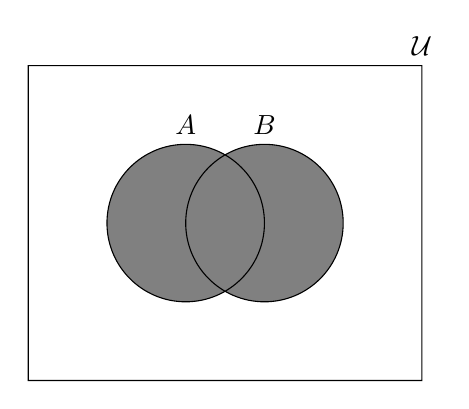
\begin{tikzpicture}[fill=gray]
	% left hand
	\scope
	(-2,-2) rectangle (2,2)
	(1,0) circle (1);
	\fill (0,0) circle (1);
	\endscope
	% right hand
	\scope
	(-2,-2) rectangle (2,2)
	(0,0) circle (1);
	\fill (1,0) circle (1);
	\endscope
	% outline
	\draw (0,0) circle (1) (0,1)  node [text=black,above] {$A$}
	(1,0) circle (1) (1,1)  node [text=black,above] {$B$}
	(-2,-2) rectangle (3,2) node [text=black,above] {$\mathcal{U}$};
	\end{tikzpicture}
	
	Intersection $A \cap B$
	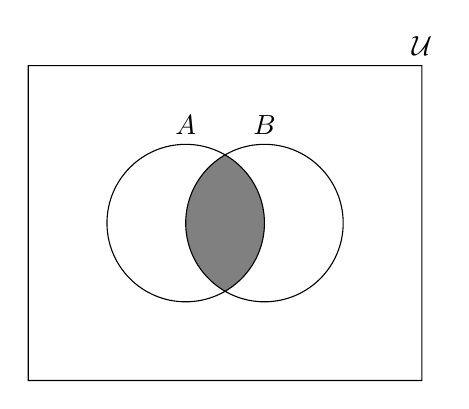
\begin{tikzpicture}[fill=gray]
	% left hand
	\scope % A \cap B
	\clip (0,0) circle (1);
	\fill (1,0) circle (1);
	\endscope
	% right hand
	\scope
	(-2,-2) rectangle (2,2)
	(0,0) circle (1);
	\endscope
	% outline
	\draw (0,0) circle (1) (0,1)  node [text=black,above] {$A$}
	(1,0) circle (1) (1,1)  node [text=black,above] {$B$}
	(-2,-2) rectangle (3,2) node [text=black,above] {$\mathcal{U}$};
	\end{tikzpicture}
	
	Difference $B-A$
	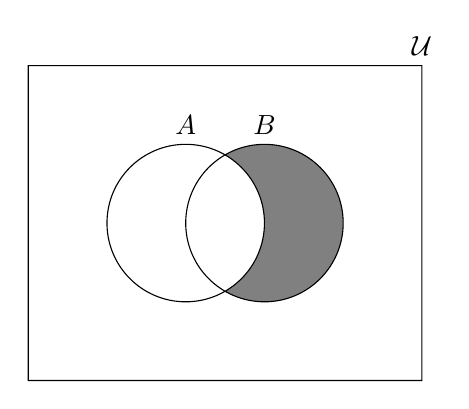
\begin{tikzpicture}[fill=gray]
	% left hand
	\scope
	(-2,-2) rectangle (2,2)
	(1,0) circle (1);
	\endscope
	% right hand
	\scope
	\clip (-2,-2) rectangle (2,2)
	(0,0) circle (1);
	\fill (1,0) circle (1);
	\endscope
	% outline
	\draw (0,0) circle (1) (0,1)  node [text=black,above] {$A$}
	(1,0) circle (1) (1,1)  node [text=black,above] {$B$}
	(-2,-2) rectangle (3,2) node [text=black,above] {$\mathcal{U}$};
	\end{tikzpicture}
\end{multicols}

\subsection{Basic Set Theory}
The formal set theory is called \textbf{Zermelo-Fraenkel Set Theory} with the \textbf{Axiom of Choice}, or simply \textbf{ZFC}. In our scope, we will simply study basic set theory.\\ \\
We will let $\mathcal{U}$ denote the universal set, or the universe of discourse, that contains all the objects in our context of discussion.\\ \\
We define the empty set to be the set that has no element, and is denoted as $\emptyset$ or $\{\}$. Mathematically,
\begin{center}
	$\forall Y \in \mathcal{U}, Y \notin \emptyset$
\end{center}
Furthermore, for all sets $S$, $\emptyset \subseteq S$, and the empty set itself is unique.\\ \\
We will go through a few more definitions:\\
\textbf{Set equality} - Two sets are equal if and only if they have the same elements\\
\textbf{Power Set} - Given any set $S$, the power set of $S$, denoted by $\mathcal{P}(S)$, or $2^S$, is the set whose elements are all the subsets of $S$. Mathematically, if $T = \mathcal{P}(S)$, then $T=\{X$ | $X \subseteq S \}$\\ \\
For any two sets $X$ and $Y$, $X$ is a subset of $Y$ and $Y$ is a subset of $X$ if, and only if, $X=Y$.\\ \\

\subsection{Operation on sets}
\subsubsection{Union}
Let $S$ be a set of sets, then we say that $T$ is the union of the sets in $S$, and write:
\begin{center}
	$T = \bigcup S = \bigcup\limits_{X\in S}X$
\end{center}
iff each element of $T$ belongs to some set in $S$.\\
That is, given $S$, the set $T$ is such that:
\begin{center}
	$T = \{y\in \mathcal{U}$ | $y \in X$ for some $X \in S\}$
\end{center}
For two sets $A, B$, we may simply write $T = A \cup B$\\\\
Some simple propositions:\\
Let $A, B, C$ be sets. Then
\begin{itemize}
	\item $\bigcup \emptyset = \bigcup\limits_{A\in \emptyset} A = \emptyset$
	\item $\bigcup\{A\} = A$
	\item $A\cup \emptyset = A$
	\item $A\cup B = B\cup A$
	\item $A\cup (B\cup C) = (A\cup B) \cup C$
	\item $A\cup A = A$
	\item $A\subseteq B \leftrightarrow A\cup B = B$
\end{itemize}

\subsubsection{Intersection}
Let $S$ be a non-empty set of sets, then we say that the intersection of the sets in $S$ is the set $T$ whose elements belong to \textit{all} the sets in $S$ and write:
\begin{center}
	$T = \bigcup S = \bigcup\limits_{X\in S}X$
\end{center}
That is, given $S$, the set $T$ is such that:
\begin{center}
	$T = \{y\in \mathcal{U}$ | $\forall X ((X\in S) \rightarrow (y \in X))\}$
\end{center}
For two sets $A, B$, we may simply write $T = A \cap B$.\\\\
Some simple propositions:\\
Let $A, B, C$ be sets. Then
\begin{itemize}
	\item $A\cap \emptyset = \emptyset$
	\item $A\cap B = B\cap A$
	\item $A\cap (B\cap C) = (A\cap B) \cap C$
	\item $A\subseteq B \leftrightarrow A\cap B = B$
\end{itemize}
Furthermore, by distributivity laws:
\begin{itemize}
	\item $A\cap (B\cup C) = (A\cap B) \cup (A\cap C)$
	\item $A\cup (B\cap C) = (A\cup B) \cap (A\cup C)$
\end{itemize}

\subsubsection{More definitions}
\begin{itemize}
	\item \textbf{Disjoint} - Let $S$ and $T$ be two sets, $S$ and $T$ are disjoint iif $S\cap T = \emptyset$
	\item \textbf{Mutually disjoint} - Let $V$ be a set of sets. The sets $T\in V$ are mutually disjoint iff every two distinct sets are disjoint: 
	$\forall X,Y \in V (X \neq Y \rightarrow X\cap Y = \emptyset)$
	\item \textbf{Partition} - Let $S$ be a set, and let $V$ be a set of non-empty subsets of $S$. Then $V$ is called a partition of $S$ iff:
	\begin{itemize}
		\item The sets in $V$ are mutually disjoint.
		\item The union of the sets in $V$ equals $S$.
	\end{itemize}
	\item \textbf{Non-symmetric Difference} -  Let $S$ and $T$ be two sets. The (non-symmetric) differnce (or relative complement) of $S$ and $T$, denoted $S-T$ or $S \ T$, is the set whose elements belong to $S$ and do not belong to $T$.\\
	$S-T = \{y \in \mathcal{U}$ | $ y\in S \land y \notin T\}$
	\item \textbf{Symmetric Difference} - Let $S$ and $T$ be two sets. The symmetric differnce of $S$ and $T$, denoted $S\ominus T$ or $S \Delta T$, is the set whose elements belong to $S$ or $T$, but not both.\\
	$S\ominus T = \{y \in \mathcal{U}$ | $ y\in S \oplus y \in T\}$
	\item \textbf{Set Complement} - Let $A \subseteq \mathcal{U}$. Then the complement of $A$, denoted $A^C$, is $\mathcal{U}-A$ 
\end{itemize}

\section{Relations}
\subsection{Introduction}
In math, relations are structures on a set that pairs any two objects that satisfy certain properties.\\ \\
We start with a few definitions:
\begin{itemize}
	\item \textbf{Ordered Pair} - Let $S$ be a non-empty set, and let $x,y$ be two elements in $S$. The ordered pair, denoted $(x,y)$ is a mathematical object in which the first element of the pair is $x$ and the second element is $y$. Two ordered pairs $(x,y)$ and $(a,b)$ are equal iff $x=a$, $y=b$.
	\item \textbf{Ordered n-tuple} - Let $n$ be a positive integer and let $x_1, x_2, \dots, x_n$ be (not necessarily distinct) elements. The ordered n-tuple, $(x_1, x_2, \dots, x_n)$ consists of $x_1, x_2,\dots, x_n$ together with the ordering. Two ordered n-tuples $(x_1, x_2, \dots, x_n)$ and $(y_1, y_2, \dots, y_n)$ are equal if and only if $x_1 = y_1$, $x_2 = y_2$, $\dots$, $x_n = y_n$
	\item \textbf{Cartesian product} - Let $S$ and $T$ be two sets. The Cartesian product (or cross product) of $S$ and $T$, denoted $S \times T$, is the set such that: $\forall X \forall Y ((X,Y) \in S \times T \leftrightarrow (X\in S) \land (Y\in T))$
	\item \textbf{Generalized Cartesian product} - Given sets $A_1, A_2, \dots, A_n$, the Cartesian product of $A_1, A_2, \dots, A_n$, denoted $A_1 \times A_2 \times \dots \times A_n$ is the set of all ordered n-tules $(a_1,a_2,\dots,a_n)$ where $a_1\in A_1, a_2\in A_2,\dots,a_n\in A_n$. If $V$ is a set of sets, we can write the Generalized Cartesian product of its elements as $\prod\limits_{S\in V}S$
\end{itemize}
\subsection{Relations}
Let $S$ and $T$ be two sets. A \textbf{binary relation} from $S$ to $T$, noted $\mathcal{R}$, is a subset of the Cartesian product $S\times T$.\\ \\
$s \mathcal{R} t$ stands for $(s,t) \in \mathcal{R}$\\
$s \cancel{\mathcal{R}} y$ stands for $(x,y) \notin \mathcal{R}$\\ \\
We introduce more definitions for binary relations:\\
Let $\mathcal{R} \subseteq S \times T$ be a binary relation from $S$ to $T$.
\begin{itemize}
	\item The \textbf{domain} of $\mathcal{R}$ is the set $Dom(\mathcal{R}) = \{s \in S$ | $\exists t \in T (s \mathcal{R} t)\}$
	\item The \textbf{image} or \textbf{range} of $\mathcal{R}$ is the set $Im(\mathcal{R}) = \{t \in T$ | $\exists s \in S (s \mathcal{R} t)\}$
	\item The \textbf{co-domain} of $\mathcal{R}$ is the set $coDom(\mathcal{R}) = T$. Note that $Im(\mathcal{R}) \subseteq coDom(\mathcal{R})$
	\item The \textbf{inverse} of the relation $\mathcal{R}$, denoted $\mathcal{R}^{-1}$, is the relation from $T$ to $S$ such that: $\forall s \in S$, $\forall t \in T$ $(t \mathcal{R}^{-1} s \leftrightarrow s \mathcal{R} t)$
\end{itemize}
Furthermore, let $S$, $T$, and $U$ be sets. Let $\mathcal{R} \subseteq S \times T$ be a relation. Let $\mathcal{R}' \subseteq T \times U$ be a relation. The \textbf{composition} of $\mathcal{R}$ with $\mathcal{R}'$, denoted $\mathcal{R}' \circ \mathcal{R}$, is the relation from $S$ to $U$ such that:
\begin{center}
	$\forall x \in S, \forall z \in U$ $(x\mathcal{R}'\circ \mathcal{R} z \leftrightarrow (\exists y \in T$ $(x \mathcal{R} y \land y \mathcal{R}' z)))$
\end{center}
In essence, $x \in S$ and $z \in U$ are related iff there exists a "path" from $x$ to $z$ via some intermediate element $y \in T$.\\ Note that composition is associative, i.e.
\begin{center}
	$\mathcal{R}'' \circ (\mathcal{R}' \circ \mathcal{R}) = (\mathcal{R}'' \circ \mathcal{R}') \circ \mathcal{R} = \mathcal{R}'' \circ \mathcal{R}' \circ \mathcal{R}$.
\end{center}
Also, $(\mathcal{R}' \circ \mathcal{R}^{-1}) = \mathcal{R}^{-1} \circ \mathcal{R}'^{-1}$\\ \\
To generalize from binary relations, let $S_i$, for $i=1$ to $n$, be $n$ sets. An \textbf{n-ary relation} on the sets $S_i$, denoted $\mathcal{R}$, is a subset of the Cartesian product $\prod_{i=1}^{n} S_i$. We call $n$ the \textbf{arity} or \textbf{degree} of the relation. In our scope, we will focus on binary relations.

\section{Properties of relations on a set}
Let $A$ be a set, and $\mathcal{R} \subseteq A \times A$ be a relation. We say that $\mathcal{R}$ is a relation \textit{on} $A$.
Furthermore,
\begin{itemize}
	\item $\mathcal{R}$ is said to be \textbf{reflexive} iff $\forall x \in A (x $ $\mathcal{R}$ $x)$
	\item $\mathcal{R}$ is said to be \textbf{symmetric} iff $\forall x, y \in A (x $ $\mathcal{R}$ $y \rightarrow y$ $\mathcal{R}$ $x)$
	\item $\mathcal{R}$ is said to be \textbf{transitive} iff $\forall x, y, z \in A ((x $ $\mathcal{R}$ $y \land y$ $\mathcal{R}$ $z) \rightarrow x$ $\mathcal{R}$ $z)$
\end{itemize}

\section{Equivalence relations}
Let $\mathcal{R}$ be a relation on a set $A$.\\
$\mathcal{R}$ is called an \textbf{equivalence relation} iff $\mathcal{R}$ is reflexive, symmetric, and transitive.\\\\
Furthermore, let $\mathcal{R}$ be an equivalence relation on a set $A$, and let $x \in A$. The \textbf{equivalence class} of $x$, denoted $[x]$, is the set of all elements $y\in A$ that are in relation with $x$. Formally,
\begin{center}
	$[x] = \{y \in A$ | $x$ $\mathcal{R}$ $y\}$
\end{center}
In general, to prove that $\mathcal{R}$ is an equivalence relation, we need to prove that it is reflexive, symmetric, and trasitive for all elements that $\mathcal{R}$ is defined on.\\ \\
We provide the following properties of equivalence classes:\\
Let $\mathcal{R}$ be an equivalence relation on a set $A$, and let $a,b$ be two elements in $A$.
\begin{itemize}
	\item Then the set of distinct equivalent classes form a partition of $A$.
	\item If $a \mathcal{R} b$ then $[a] = [b]$.
	\item Then either $[a] \cap [b] = \emptyset$ or $[a] = [b]$
\end{itemize}
Now, lets work backwards from a partition: Given a partition $S_1, S_2,\dots$ of a set $A$, then there exists an equivalence relation $\mathcal{R}$ on $A$ whose equivalence classes make up precisely that partition.

\subsubsection{Additional definitions}
Let $A$ be a set. Let $\mathcal{R}$ be a relation on $A$. The \textbf{transitive closure} of $\mathcal{R}$, denoted $\mathcal{R}^t$, is a relation that satisfies these three properties:
\begin{enumerate}
	\item $\mathcal{R}^t$ is transitive.
	\item $\mathcal{R} \subseteq \mathcal{R}^t$.
	\item If $S$ is any other transitive relation such that $\mathcal{R} \subseteq S$, then $\mathcal{R}^t \subseteq S$.
\end{enumerate}
Also, $\mathcal{R}^t = \bigcup\limits_{i=1}^{\infty}\mathcal{R}^i$\\ \\
Note that the transitive closure is the \textit{smallest} superset that is transitive. Similar definitions can be made for reflexive closures and symmetric closures of a relation.\\ \\
Furthermore, we adopt the following notation for the composition of $\mathcal{R}$ with itself:
\begin{itemize}
	\item $\mathcal{R}^1 \triangleq \mathcal{R}$
	\item $\mathcal{R}^2 \triangleq \mathcal{R} \circ \mathcal{R}$
	\item $\mathcal{R}^n \triangleq \underbrace{\mathcal{R} \circ \dots \circ \mathcal{R}}_{n} = \odot_{i=1,2,\dots, n}\mathcal{R}$
\end{itemize}

\section{Partial and Total Orders}
Let $\mathcal{R}$ be a relation on a set $A$.\\
$\mathcal{R}$ is said to be \textbf{anti-symmetric} iff
\begin{center}
	$\forall x \in A, \forall y \in A ((x\mathcal{R}y \land y\mathcal{R}x) \rightarrow x = y)$
\end{center}
Thus, $\mathcal{R}$ is said to be a \textbf{partial order} iff it is reflexive, \textit{anti-symmetric}, and transitive.\\
We denote a partial order by the symbol $\preceq$. A set $A$ is called a partially ordered set (or poset) with respect to a relation $\preceq$ iff $\preceq$ is a partial order relation on $A$.\\ \\
Let $\preceq$ be a partial order on a set $A$. Elements $a, b$ of $A$ are said to be \textbf{comparable} iff either $a\preceq b$ or $b \preceq a$. Otherwise, $a$ and $b$ are called \textbf{noncomparable}.\\
We then say that $\preceq$ is a \textbf{total order} iff 
\begin{center}
	$\forall x,y \in A (x \preceq y \lor y \preceq x)$
\end{center}
In other words, $\preceq$ is a total order if $\preceq$ is a partial order and all $x, y$ are comparable.\\ \\
We further extend the following definitions:\\
Let $\preceq$ be a partial order on a set $A$.
\begin{itemize}
	\item An element $x$ is a \textbf{maximal element} iff $\forall y \in A (x \preceq y \rightarrow x = y)$
	\item An element, usually denoted $\top$, is the \textbf{maximum element} iff $\forall x \in A (x \preceq \top)$
	\item An element $x$ is a \textbf{minimal element} iff $\forall y \in A ( y\preceq x \rightarrow x = y)$
	\item An element, usually denoted $\bot$, is the \textbf{minimum element} iff $\forall x \in A (\bot \preceq x)$
\end{itemize}
Hence, let $\preceq$ be a total order on a set $A$. $A$ is \textbf{well ordered} iff every non-empty subset of $A$ contains a minimum element. Mathematically,
\begin{center}
$\forall S \in \mathcal{P}(A)$ $(S\neq \emptyset \rightarrow$ $(\exists x \in S$ $\forall y \in S$ $(x\preceq y)))$
\end{center}

\end{document}